\section{PIT Histograms}

This section shows the PIT histograms of the different models 
broken down into the predictions for each hour.

\begin{figure}[h]%
    \centering
    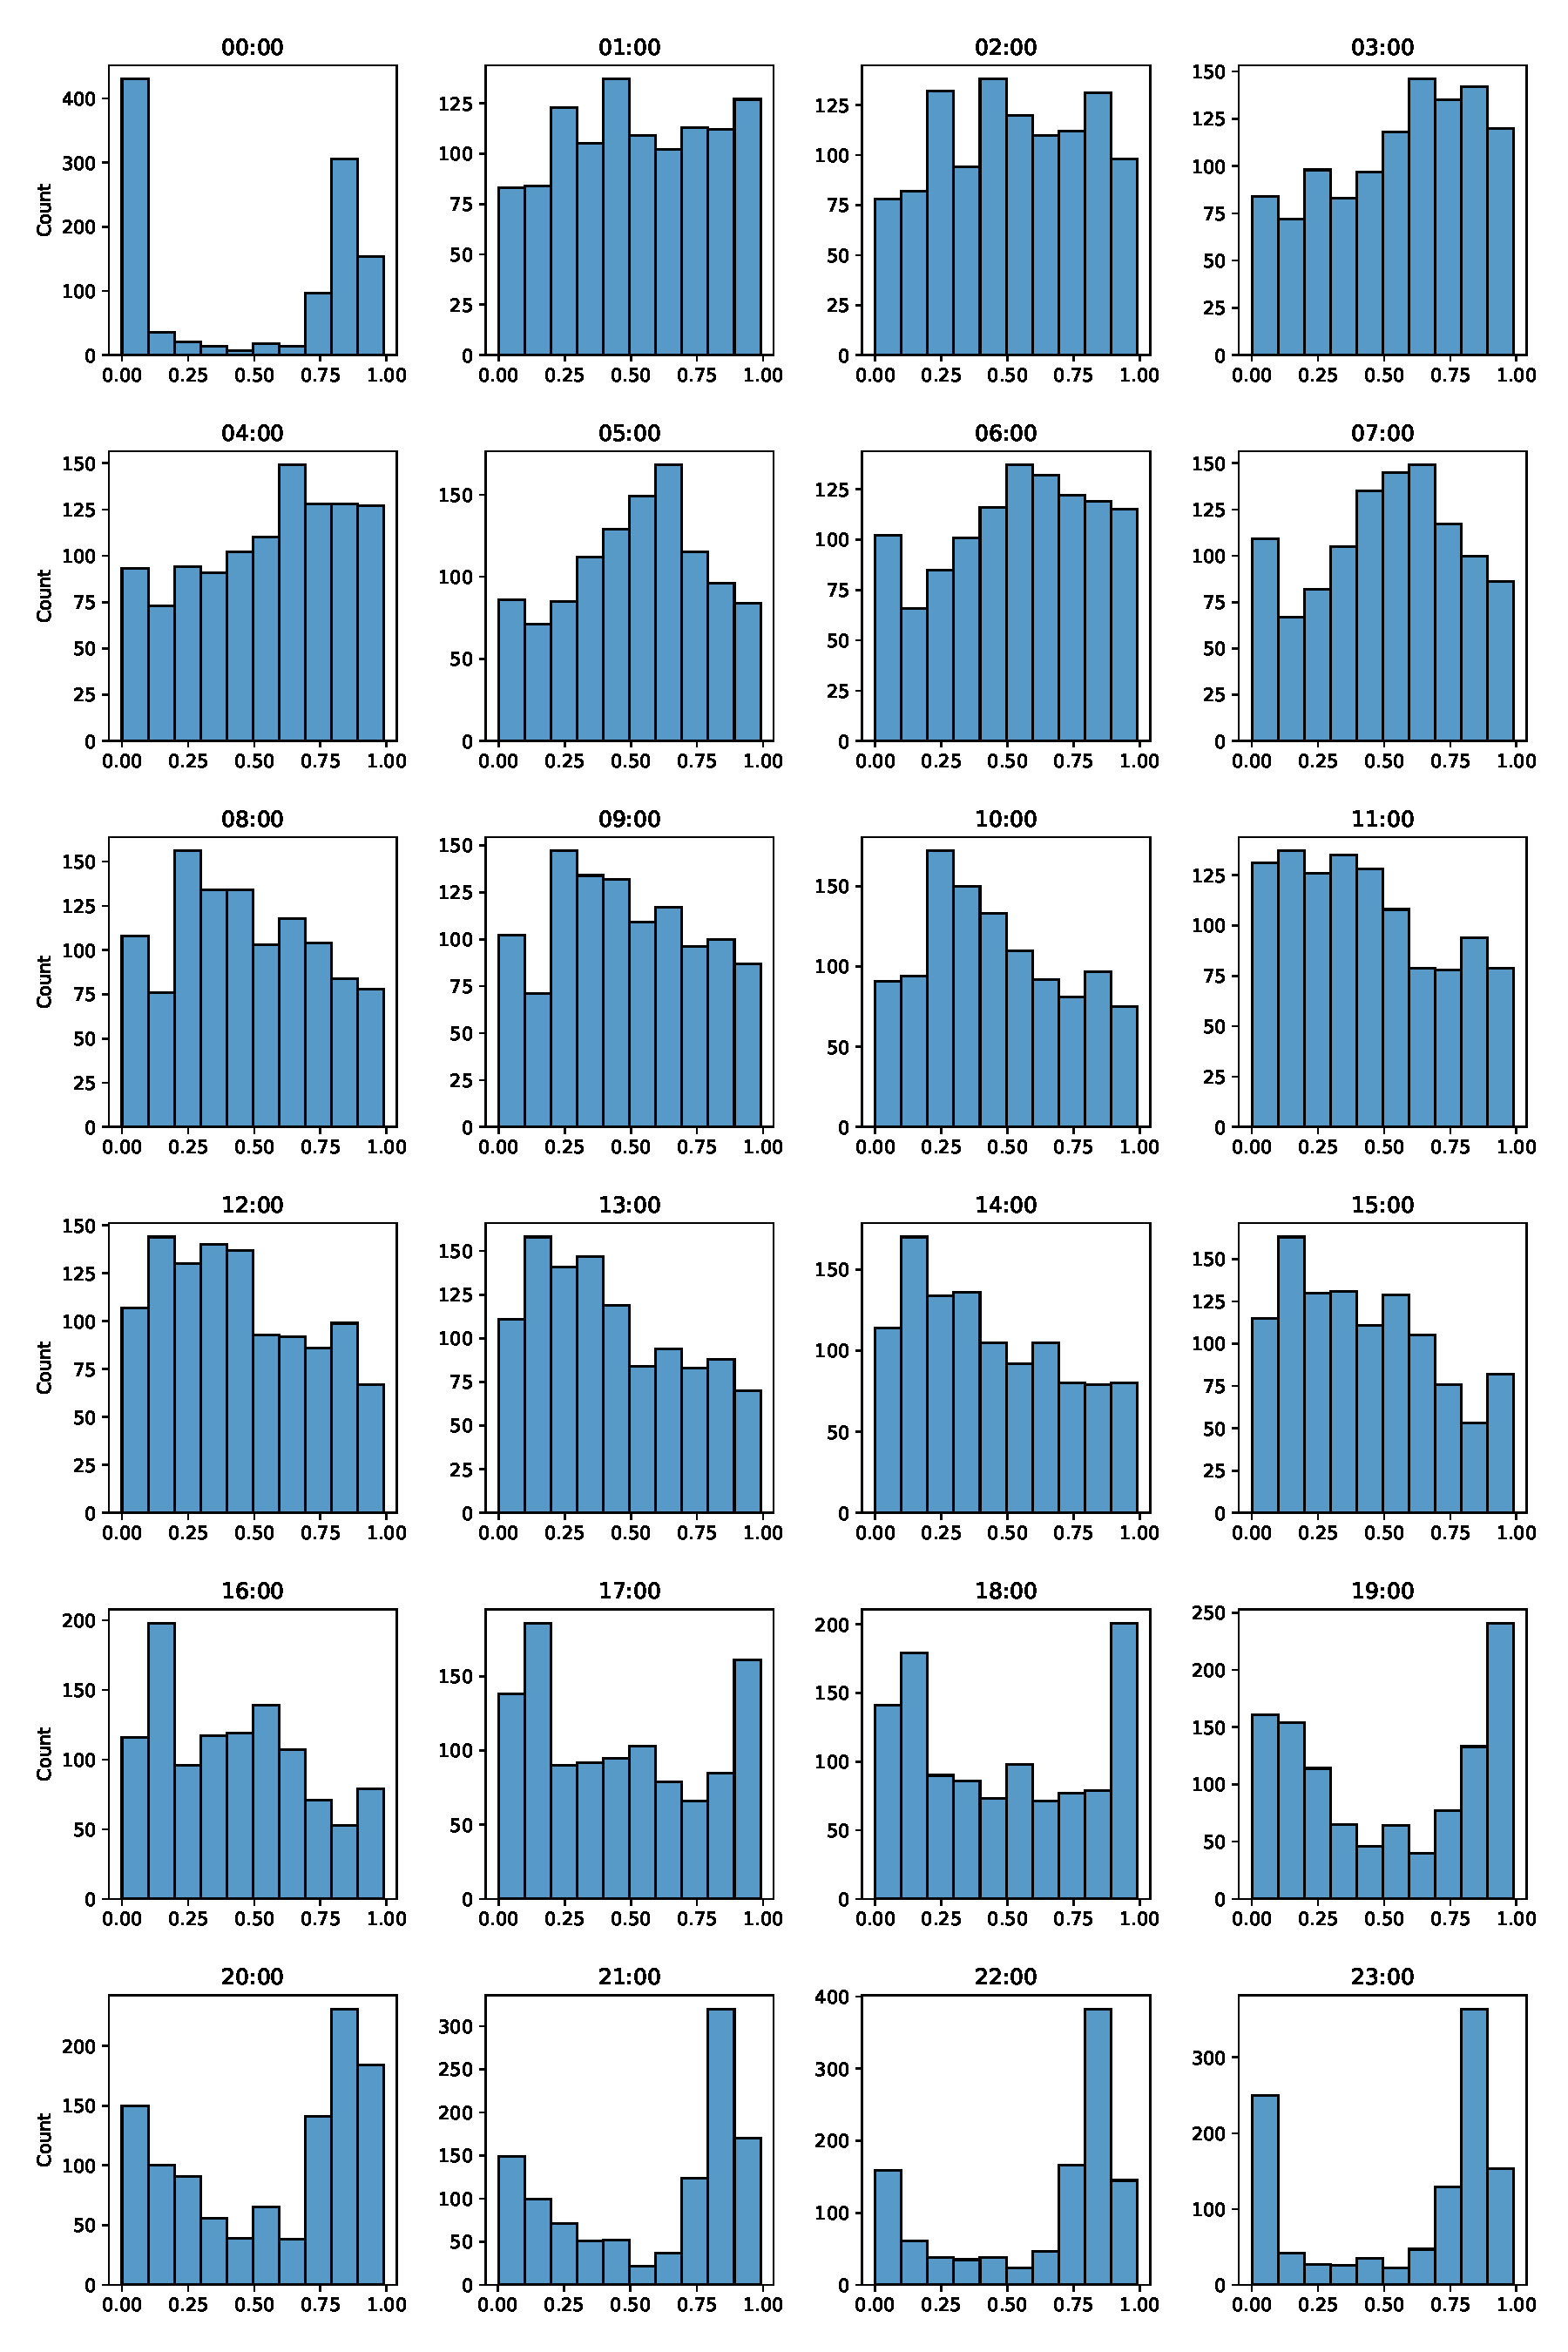
\includegraphics[width=\textwidth]{plots/pit/pit_by_hour_qrf.pdf}
    \caption[PIT histograms QRF]{PIT histograms of QRF. Since the model performs differently 
    in each hour, the PIT histogram is broken down into each hour.}%
    \label{fig:pit-qrf-by-hour}%
\end{figure}

\begin{figure}[h]%
    \centering
    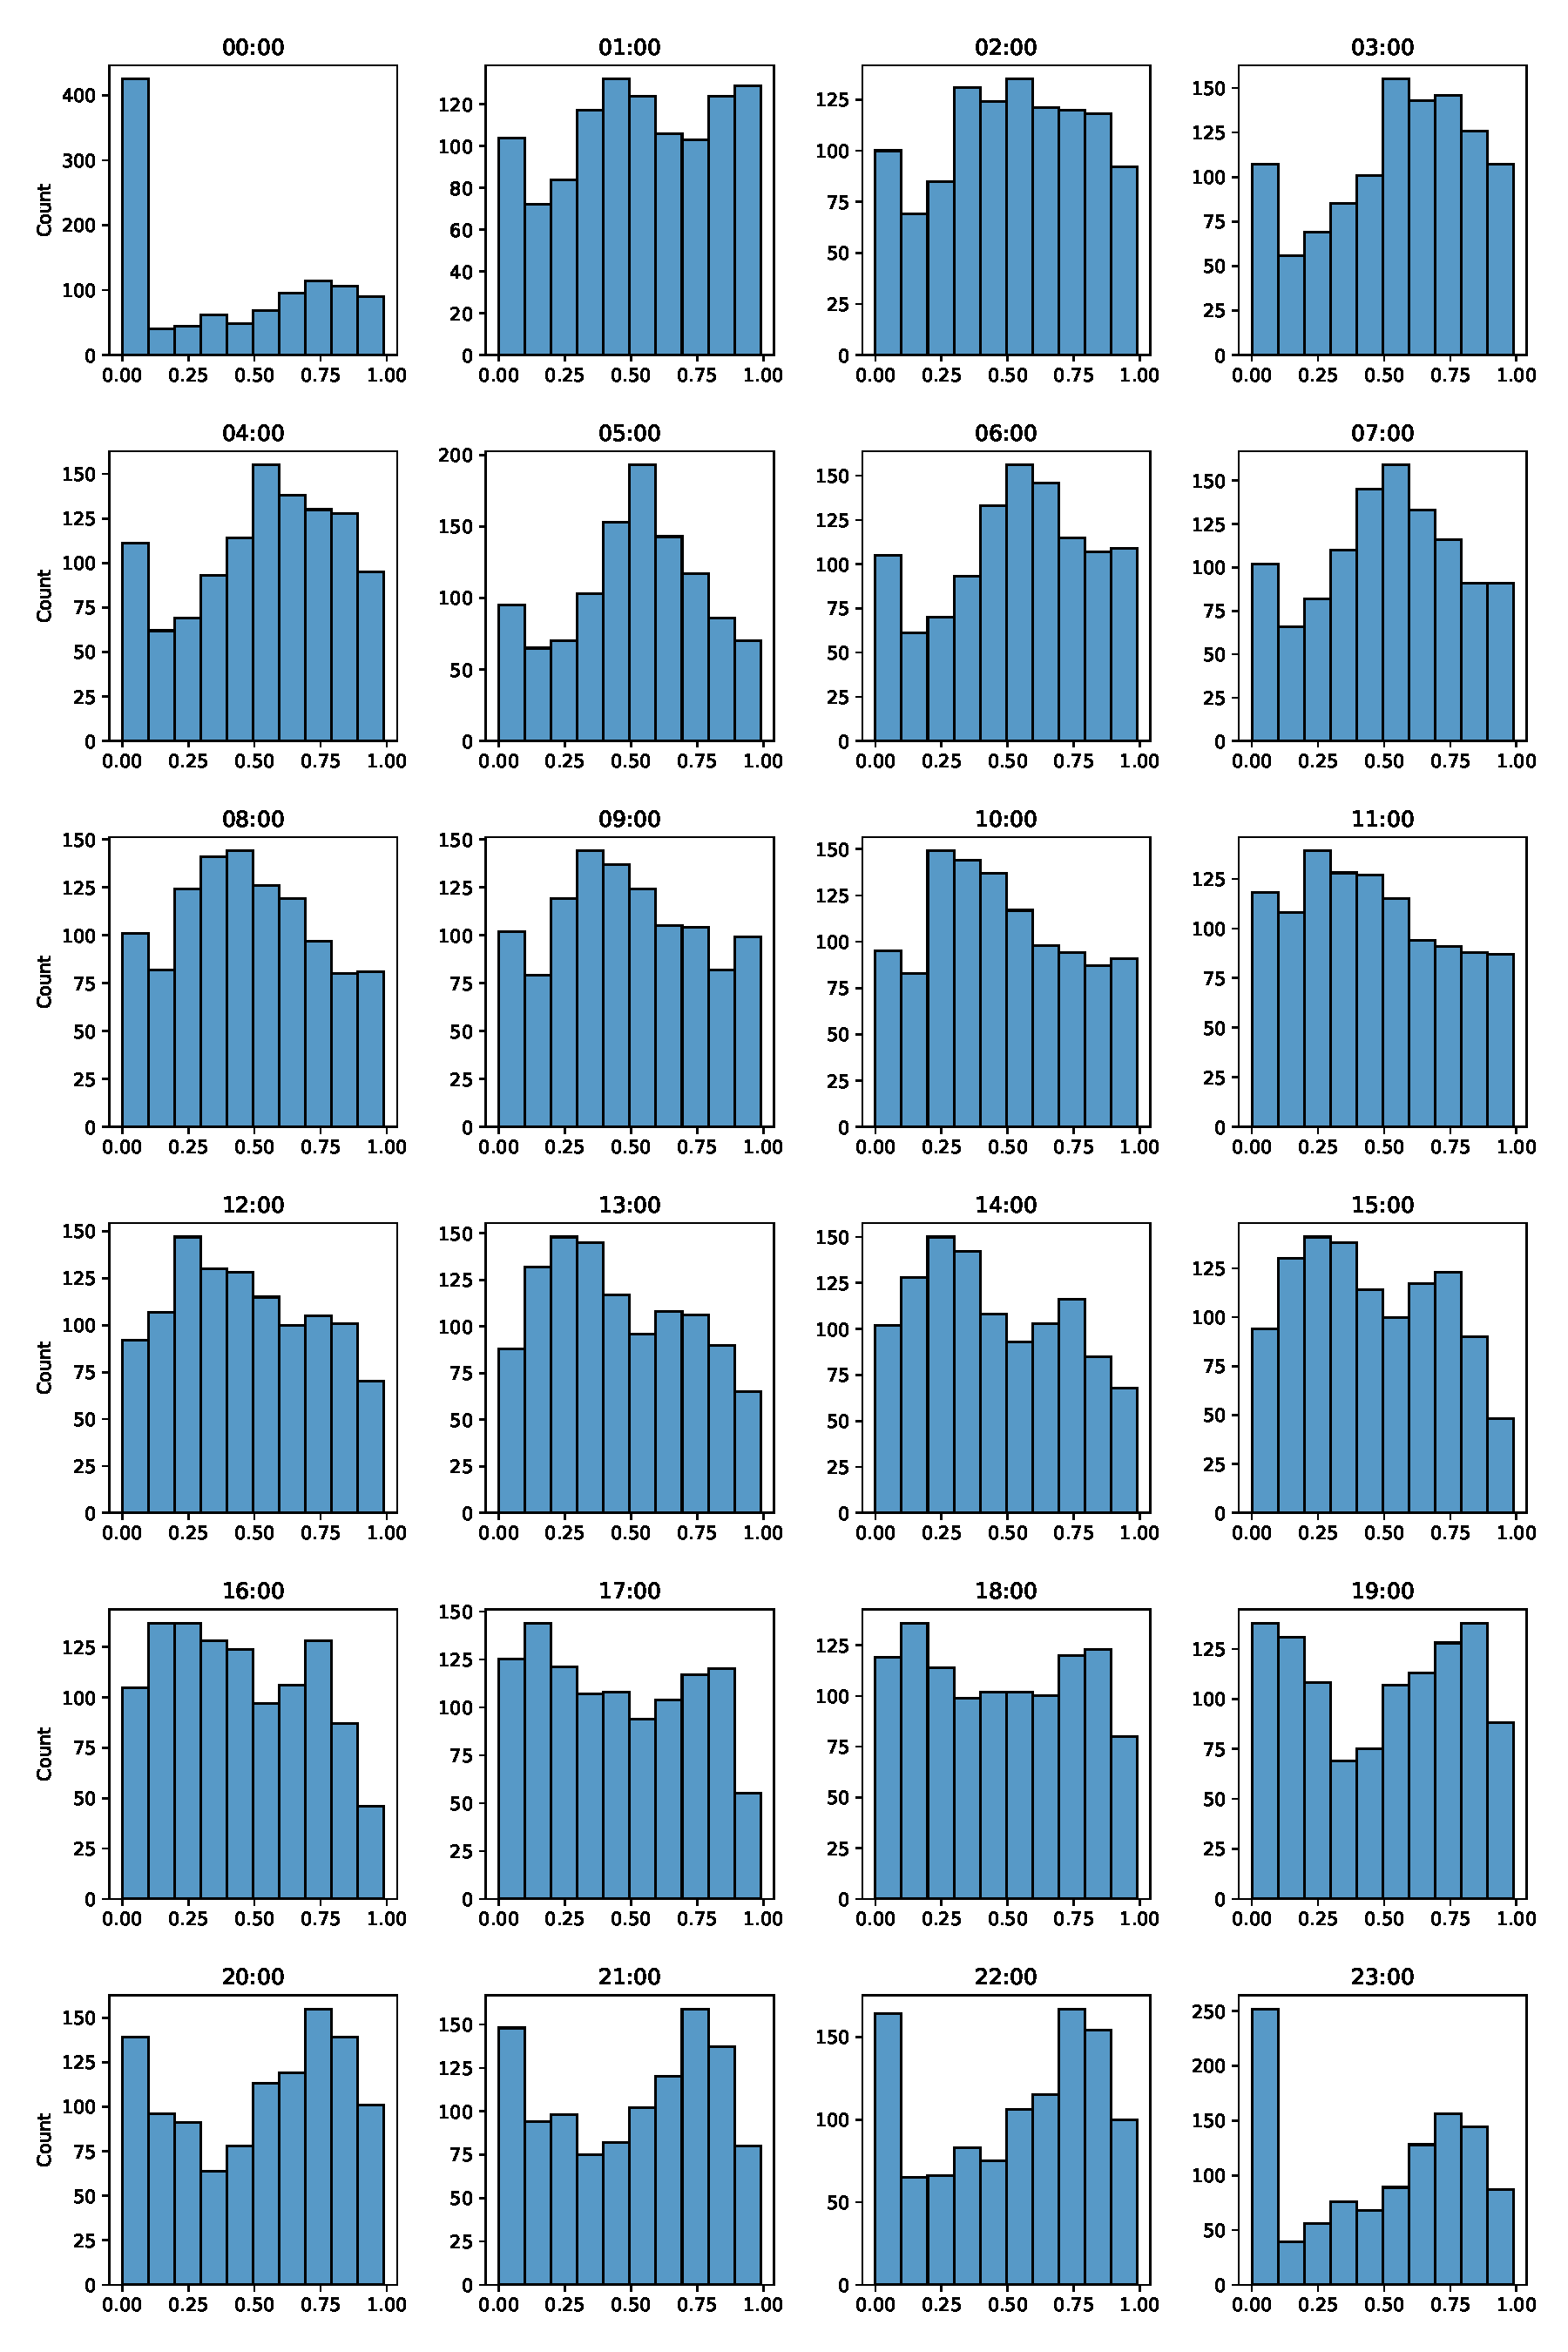
\includegraphics[width=\textwidth]{plots/pit/pit_by_hour_nnqf.pdf}
    \caption[PIT histograms NNQF]{PIT histograms of NNQF. Since the model performs differently 
    in each hour, the PIT histogram is broken down into each hour.}%
    \label{fig:pit-nnqf-by-hour}%
\end{figure}

\begin{figure}[h]%
    \centering
    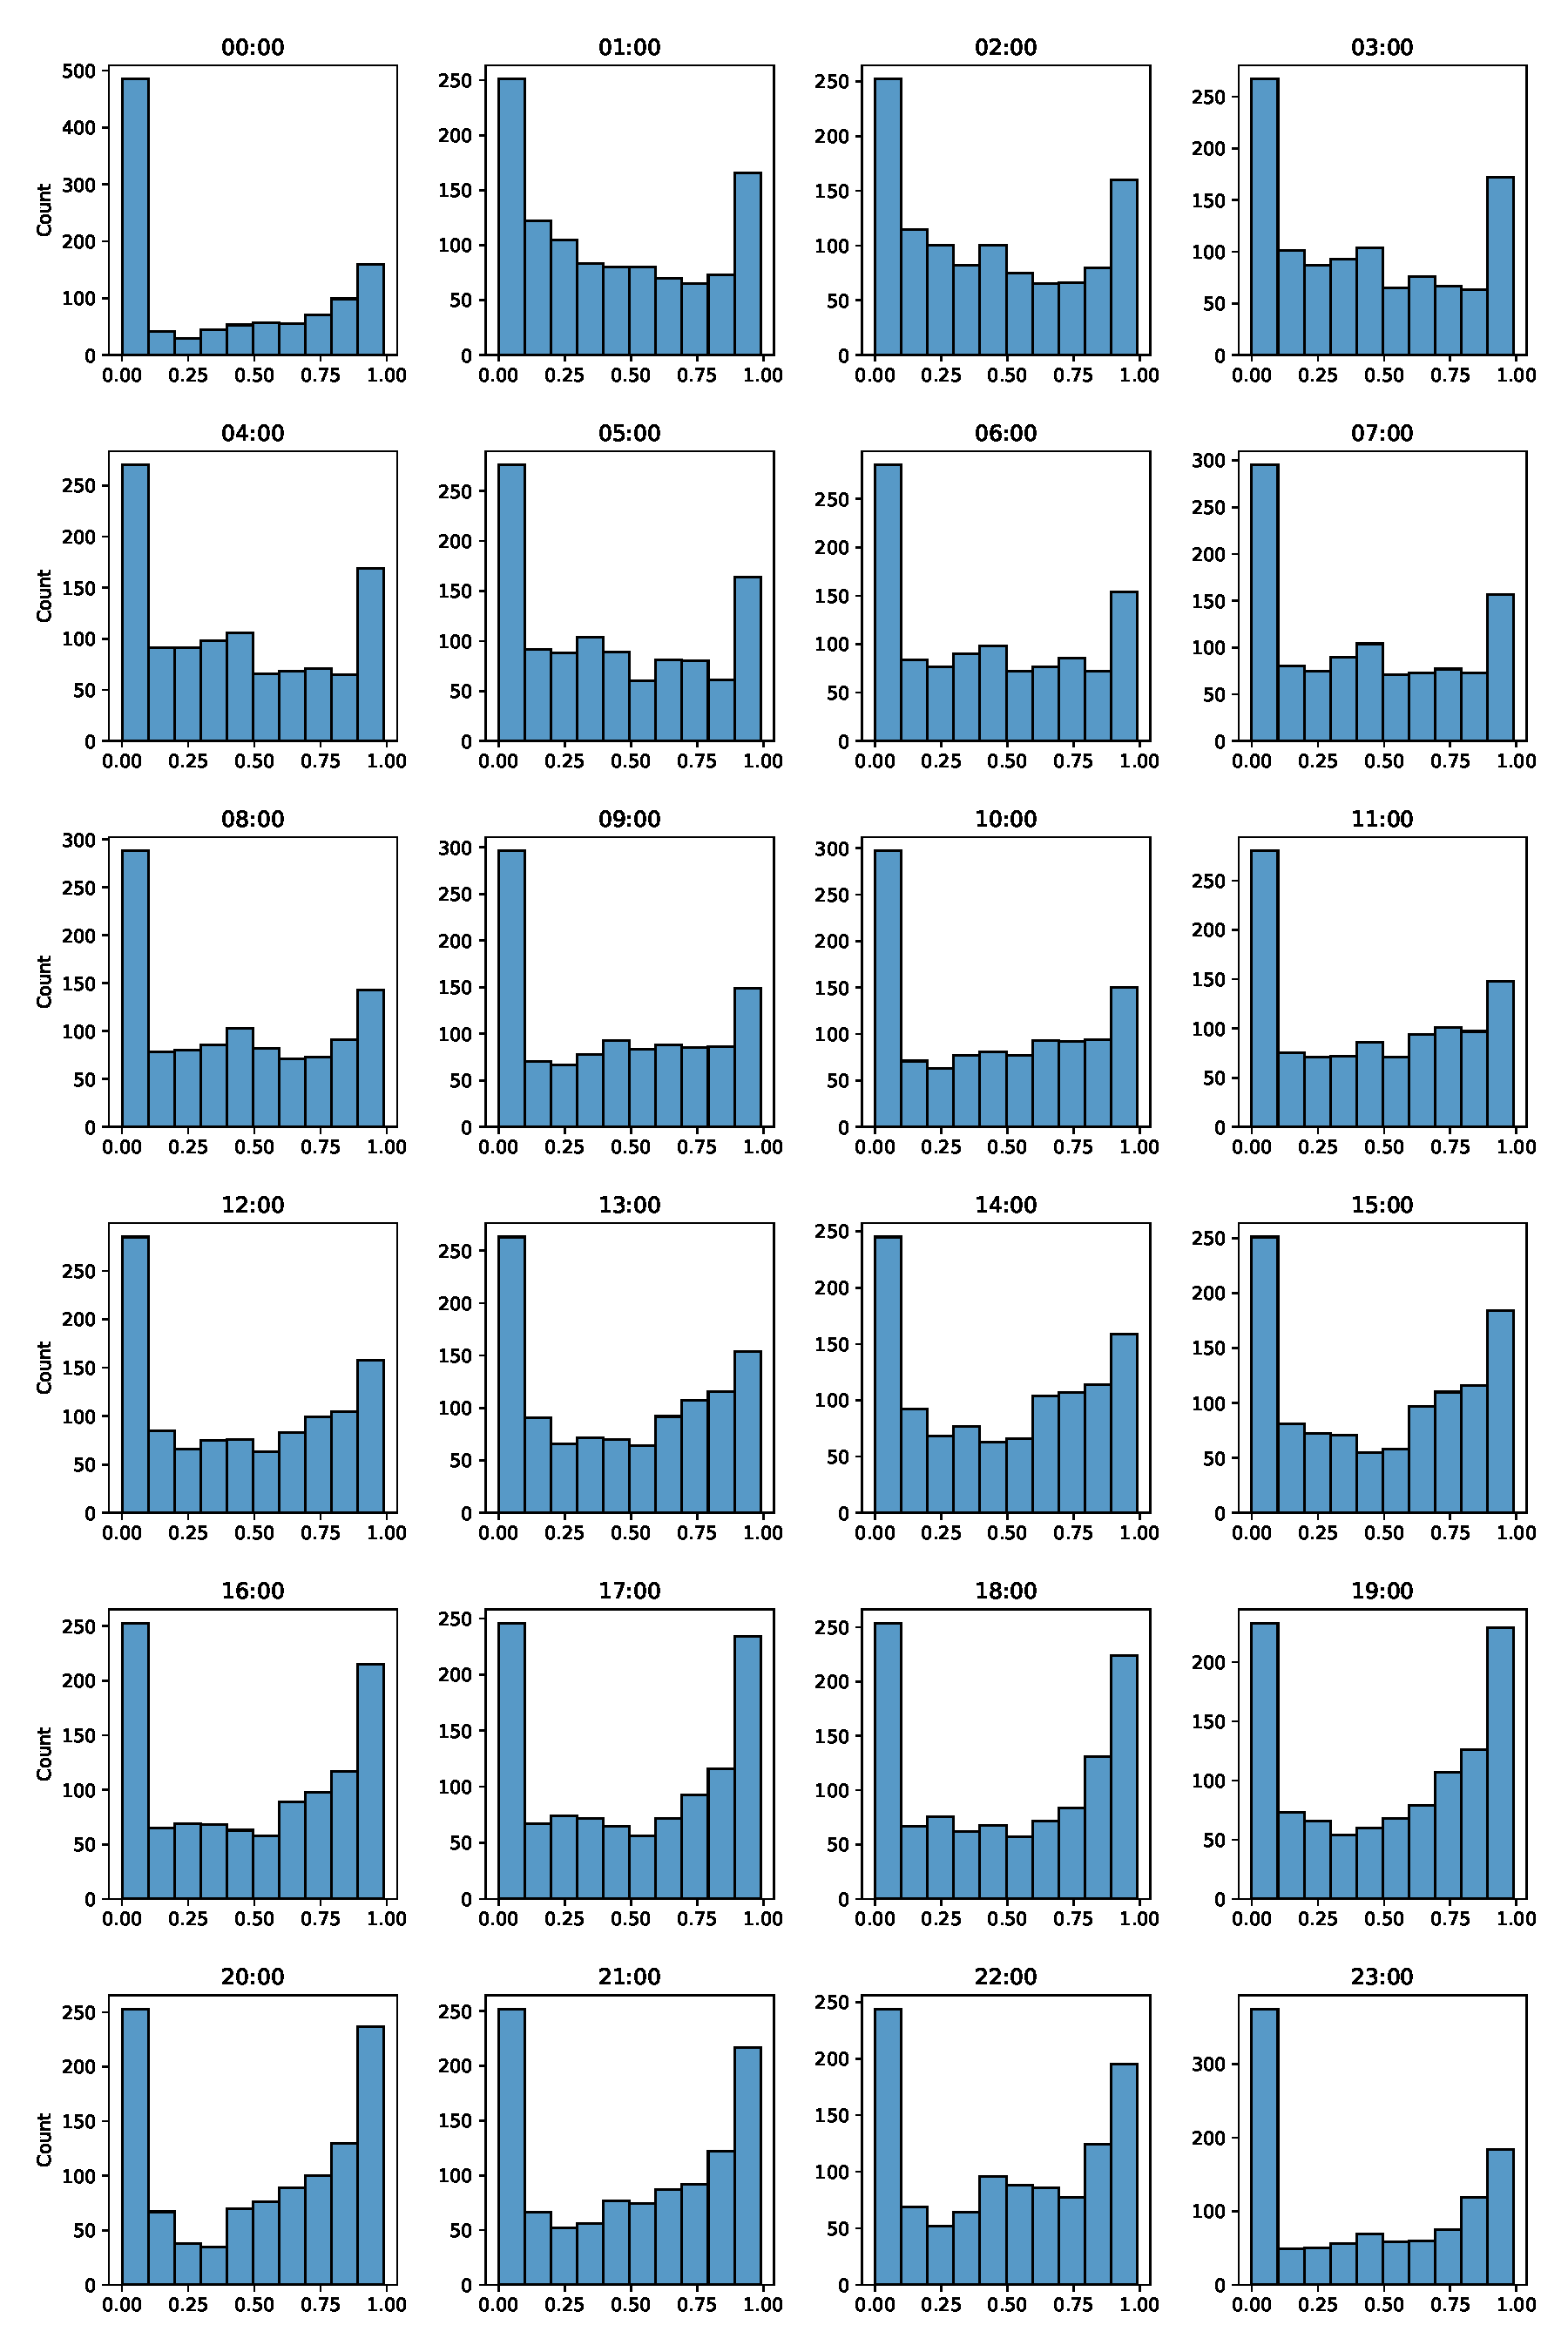
\includegraphics[width=\textwidth]{plots/pit/pit_by_hour_deepar.pdf}
    \caption[PIT histograms DeepAR]{PIT histograms of DeepAR. Since the model performs differently 
    in each hour, the PIT histogram is broken down into each hour.}%
    \label{fig:pit-deepar-by-hour}%
\end{figure}

\begin{figure}[h]%
    \centering
    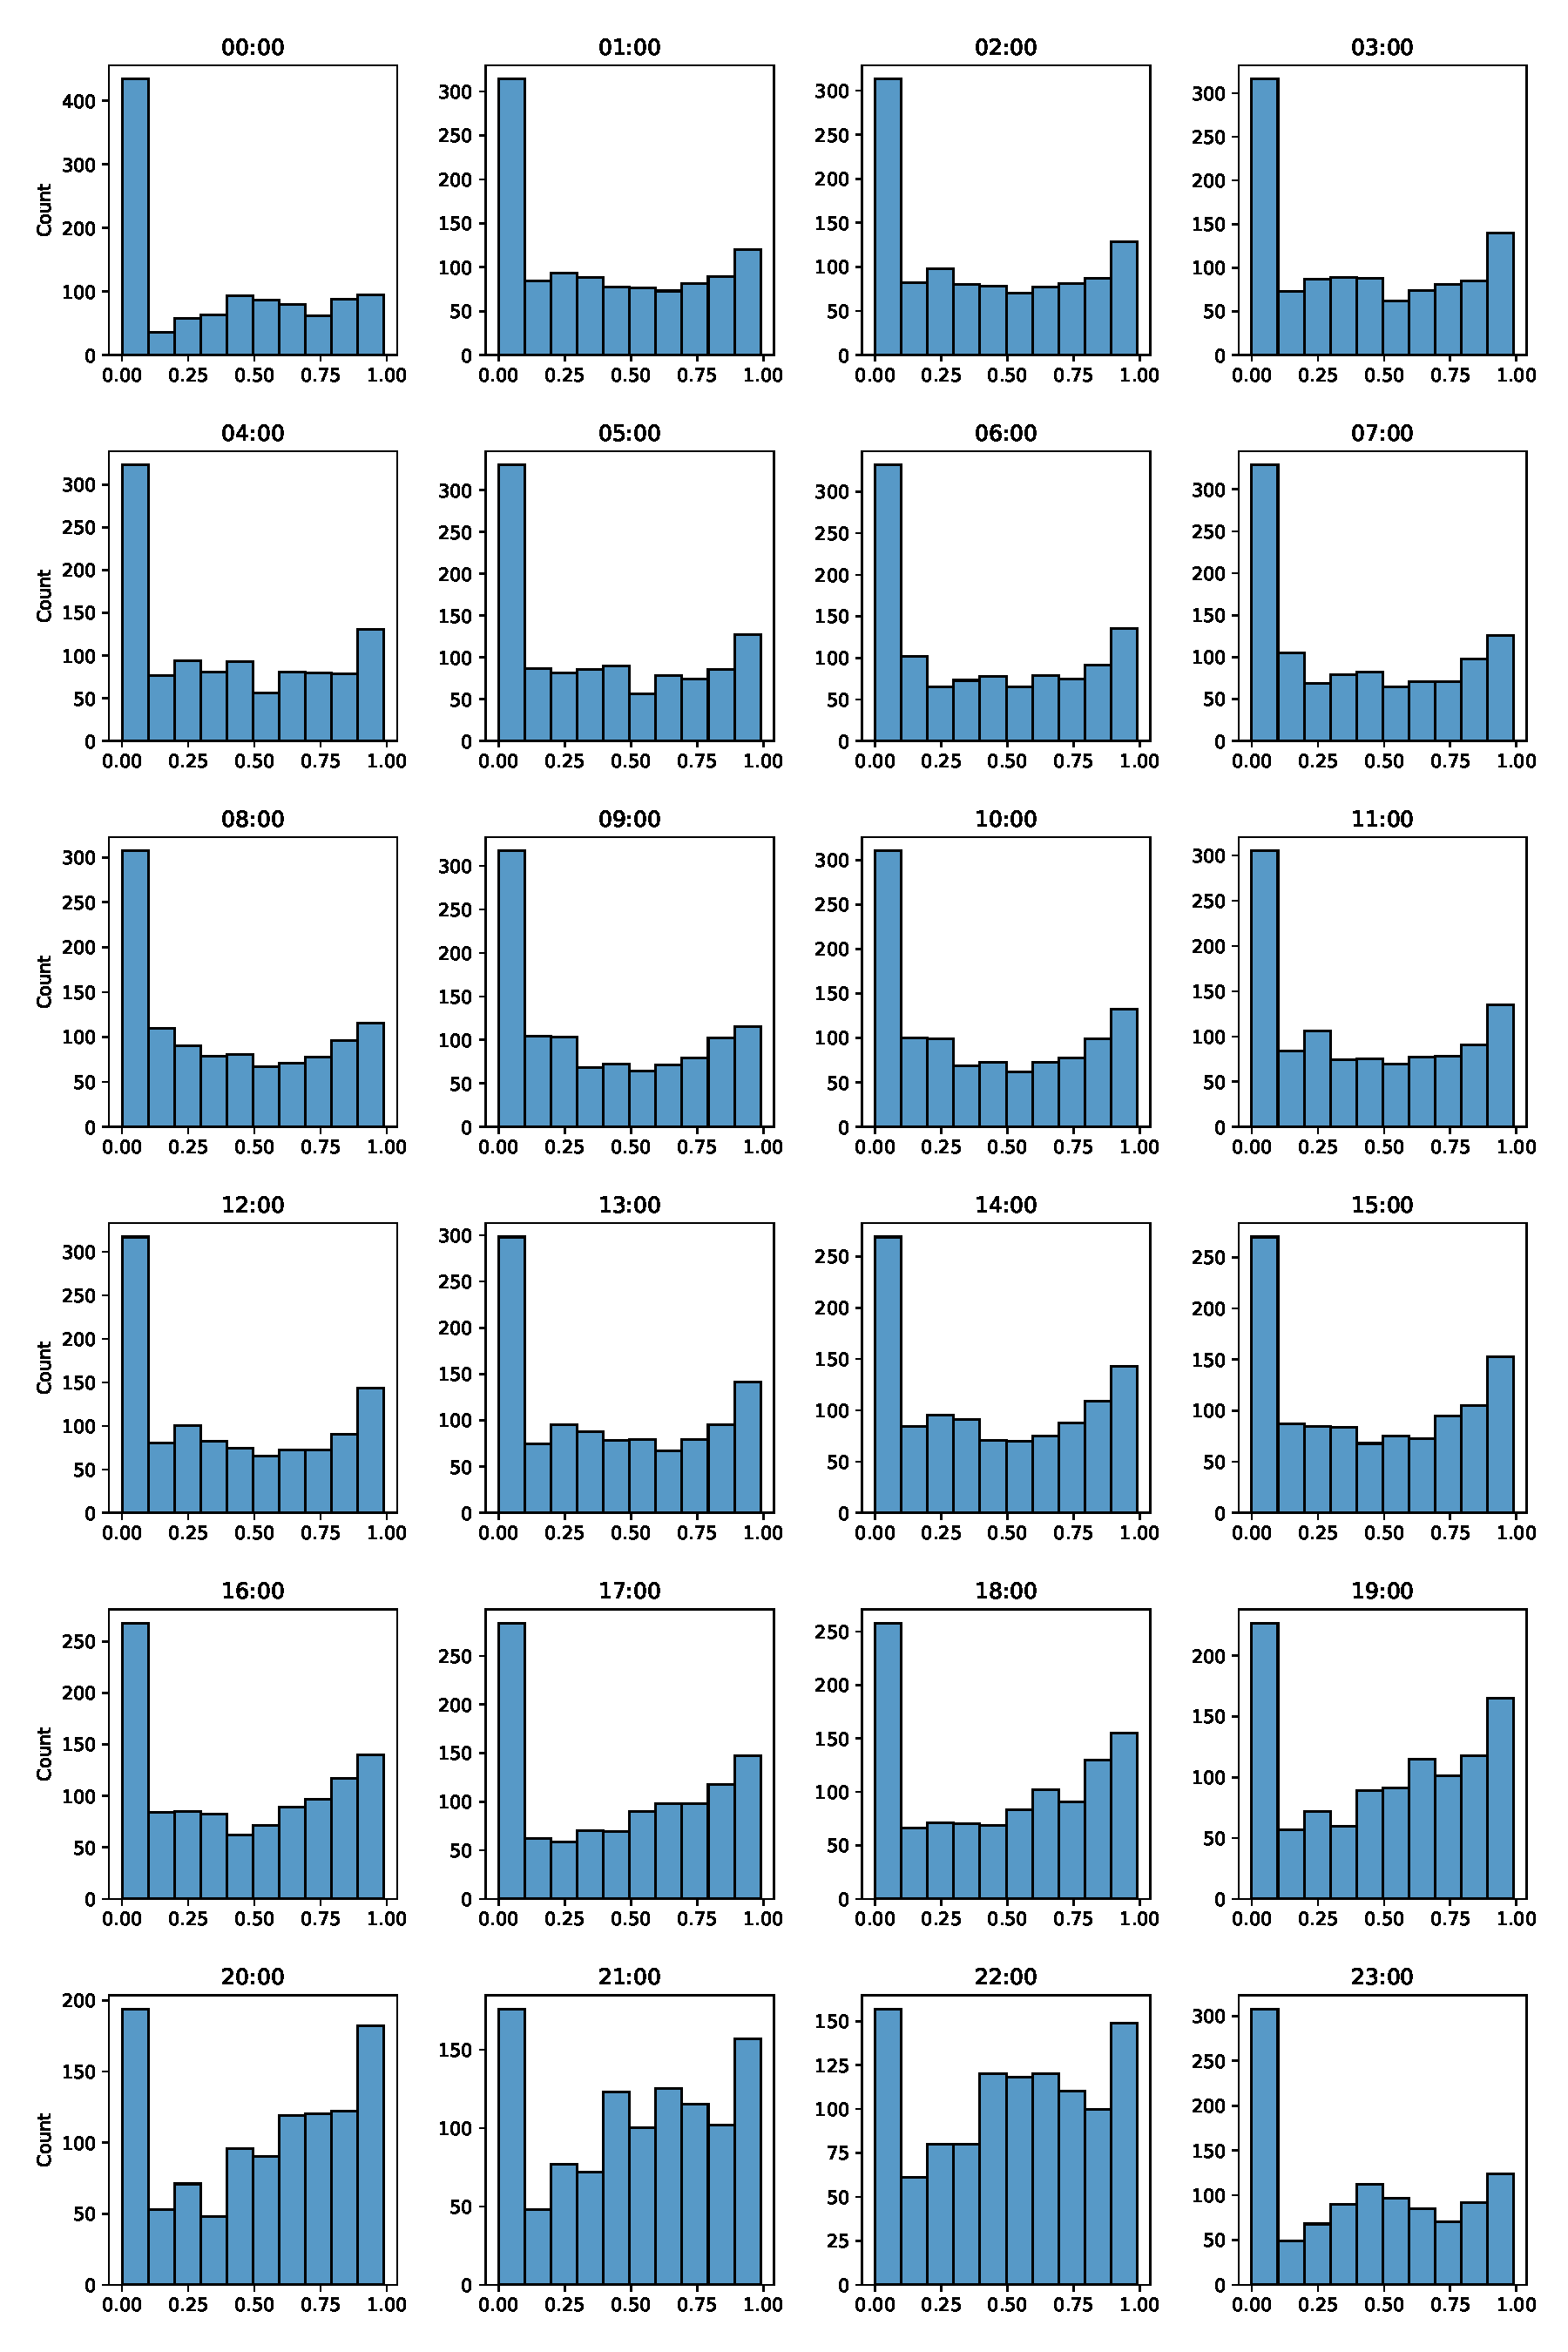
\includegraphics[width=\textwidth]{plots/pit/pit_by_hour_sqf-rnn.pdf}
    \caption[PIT histograms SQF-RNN]{PIT histograms of SQF-RNN. Since the model performs differently 
    in each hour, the PIT histogram is broken down into each hour.}%
    \label{fig:pit-sqf-rnn-by-hour}%
\end{figure}